\begin{figure}[H]
\centering
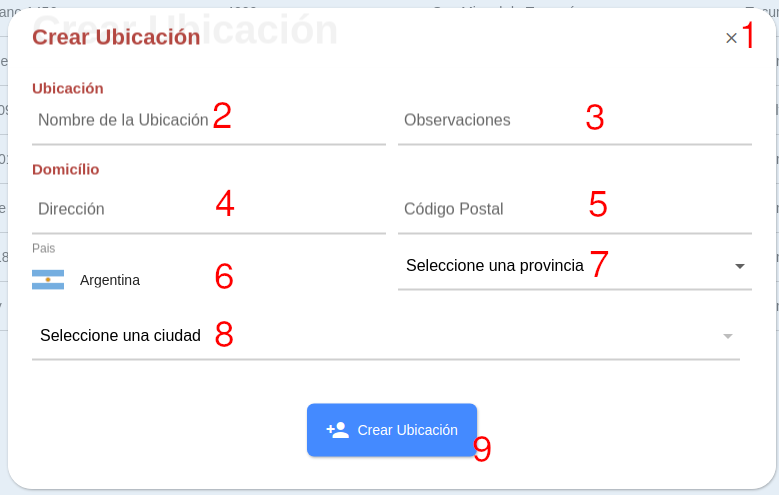
\includegraphics[width=\textwidth,height=\textheight,keepaspectratio]{Escenarios/AD-38-00}
\caption{Escenario - AD-38-00}
\label{fig:AD-38-00}
\end{figure}

Este escenario permite crear una ubicación. Con el botón \textbf{AD-38-01} se podrá volver al escenario \textbf{AD-37-00}. Se debe ingresar el nombre de la ubicación en \textbf{AD-38-02}, las observaciones que se deseen realizar en \textbf{AD-38-03}, el domicilio en \textbf{AD-38-04}, código postal en \textbf{AD-38-05} y las listas desplegables \textbf{AD-38-06}, \textbf{AD-38-07} y \textbf{AD-38-08}  permiten indicar el pais, provincia y ciudad, respectivamente, del domicilio que se indicó. El botón \textbf{AD-38-10} permite crear la ubicación con los valores indicados en los campos y listas desplegables mencionadas anteriormente.
\clearpage
